
\documentclass[pdftex,12pt,final,a4paper]{report}

% This is for norwegian letters (æøå)
\usepackage[utf8]{inputenc}

% This is to use \includegraphics to include the domain model
\usepackage[pdftex]{graphicx}

%\usepackage{setspace}
%\onehalfspace

% Use to create acronym list
\usepackage{acronym}
% A package that supports a lot of math symbols
\usepackage{amssymb,amsmath}
% Times font
\usepackage{times}
% This enables multirows in tables
\usepackage{multirow}
%enable float on placement on figures and tables
\usepackage{float}
%This package enables active links
\usepackage[pdftex]{hyperref}
\hypersetup{
    colorlinks,%
    citecolor=black,%
    filecolor=black,%
    linkcolor=black,%
    urlcolor=black
}



% For pseudocode and algorithms
%\usepackage{algorithmicx}
%\usepackage{algorithmic}
%\usepackage{algorithm}

%\usepackage{algorithm}
%\usepackage{algpseudocode}


% This adds line breaks between paragraphs
\setlength{\parskip}{0.10in}

% This sets indent length
\setlength\parindent{0pt}

% This enables fancy header
\headheight=14.5 pt
\usepackage{fancyhdr}
\pagestyle{fancy}
\fancyhead[L]{\leftmark}
\fancyhead[R]{}

% Enables UiA frontpage
\usepackage{uiafrontpage} 

%Enables subfigures
%\usepackage{subfig}


%%%%%%%oursss
\usepackage[USenglish]{babel}
%\usepackage{qtree}
\usepackage{verbatim}

%\usepackage[toc,page]{appendix}


\author{Håkon Bakkevig Steinsholt \\
Enok K. Eskeland \\
Leonard Loland \\
Daniel Aasen \\
Charika Samangi Perera Kukulage \\
Mahsa Hassankashi }

%\supervisor{Ole-Christoffer Granmo}

% select logo to use
\titlelogo{introduction/graphics/uia_logo.jpg}





\begin{document}

\title{Crisis Mapping}
\maketitle

\vspace{2in}
\begin{abstract}
Crisis mapping is a concept to help crisis management teams to determine the best course of action in a changing or evolving crisis situation in order to help people and save more lives. This report describes how mobile phone sensors can be used to measure, interpret and visualize a fire crisis situation. An interactive simulator was especially designed for this project to provide sensor readings affected by environmental parameters such as wind and humidity. These individual readings were used in the Gaussian Processes Regression (GPR) to estimate the area and magnitude of the fire. The kernel function of the GPR was expanded to include wind in the distance vectors. The overall system performance were visualized by putting the actual situation from the simulator together with the estimated situation from the GPR. The final results of this work shows acceptable accuracy and serve as a proof-of-concept that mobile phones can be used to map fire crisis situation. 
\end{abstract} 





%\include{preface}
%\include{thesisDefinition}

% Create table of contents 
\tableofcontents 

\listoffigures

%\listoftables

%\listofalgorithms

%Definition list
%\pagebreak
%\thispagestyle{plain}
%\begin{Huge}
%\label{definitions}
%\begin{flushleft}

%\bf Definition list
%\end{flushleft}
%\end{Huge}

%\begin{description}

%\end{description}

%\chapter{Introduction}

\section{Background}

Crisis Mapping is the process of collecting, analyzing and visualizing crisis data for further crisis management. The goal is to provide better real time decision support to determine the best course of action in a changing or evolving crisis environment. This in turn provide help to crisis victims and save more lives.

In 2010, a major earthquake crisis struck Haiti. The shock measured 7.0 on the moment magnitude scale (MMS) and was followed by another 52 aftershocks of 4.0 MMS or higher over 12 days. 1 517 000 people and their dependents were affected. People were in need of housing, food and medical attention. Mapping these needs would improve further crisis management \cite{}.

The needs on Haiti were mapped by Ushahidi, an open source software. This software collects, analyzes and visualizes data from social media, text messages and more. The Haiti government took advantage of this software and allowed crisis victims and bystanders to report needs to temporary web services and text message services. These services together with Ushahidi provided a crisis map that aided the government to send help where it was needed \cite{}.

Today, researchers are investigating how to use mobile phone sensors to map crisis situations. Many mobile phones have built-in sensors such as microphones, accelerometers, gyroscopes, barometers and GPS. In theory, these sensors can be used to detect earthquakes, fires, explosions, collisions and other crisis situations by reading abnormal magnitudes or patterns in sound, acceleration, air pressure and temperature. Mobile phones can be used to report this abnormality to a central crisis mapping system and possibly aid further crisis management.

\section{Problem Statement}

CISTECH of the University of Agder proposed a basic project about crisis mapping using mobile phones. Because crisis mapping is a general term and includes a broad range of different crisis situations, we had to narrow down the goal of the project. After consulting with our supervisor, the final goal was to create a prototype crisis mapping system that could detect fire using mobile phone sensors. We chose fire in specific because it can change or evolve over time. However, the chosen topic does not come without a set of practical limitations.

Given the project goal, we focused on two main problems that had to be solved. Firstly, fires had to be simulated. There was no way to justify starting real fires to gather this data. Simulating fire is challenging because fire spreads based several factors such as wind, heat, humidity and other over time. Secondly, mobile phone sensors do only report readings at their location and do not cover burning areas without nearby sensors. Uncovered areas have to be guesstimated.

\section{Literature Review}

\subsection{A Survey of Mobile Phone Sensing}

The field of mobile phone sensing is rapidly expanding. The accelerometer in a smart phone can determine whether the user is walking, running or standing still. The microphone can collect audio. The light sensors can determine whether the phone is in a pocket or not and the barometer can determine air pressure. In addition data can be combined from different sensors to make assumptions, for instance a phone can sense that a user is walking down a hill and in which direction he is going. Specialized sensors have also been used to measure air pollution and could perhaps be used to detect explosive residue.

There are many issues with properly utilizing and gathering data. First of all a large amount of users to properly test a system is needed. This can be solved by distributing the application via the App stores and providing an incentive for the users to use it. Second there are huge privacy issues with listening in on private conversations using the microphone and tracking the user via the GPS. This can somewhat be fixed by calculating any result on the phone and sending only the results, however this would require more resources from the phone and would likely limit battery time or performance. Some studies have shown that sensing systems have reduced the standby time by significant amounts, vastly affecting the user experience.

Creating a system that produce accurate results may also be slightly problematic as vendors did not foresee the use of their sensors in new applications. The sensor sampling rate varies based on the CPU load and the API and OS does not support complete access to the sensors. However, as the mobile phone sensing field is growing vendors are likely to catch on and provide better sensors and sensor support in future releases.

Moreover, it is also difficult to create a program that fully accounts for all possible instances. Explosives used in demolition and terrorism both create the same or similar sound and gun fire while hunting sounds the same as gun fire in a super marked. A phone also needs to know if it is currently inside a container where the sound might be suppressed, in which case the system might become more sensitive to sound. This in turn can be somewhat solved by using light or proximity sensors however there might be cases where the phone is placed in an unusual location and therefore provides inaccurate results.

\subsection{Distributed Perception Networks for Crisis Management}

Distributed Perception Networks for Crisis management (2006) focuses on the fusion of information gathered from fixed sensors and human perception. The fixed sensors are few and scarcely distributed in an area where a crisis could have devastating consequences. Endsley’s model tells that first comes perception, then comprehension and projection. The paper focuses on combining the perception of humans and the fixed sensors to create a clear picture of the situation. For example when the sensors are picking up dangerous levels of ammonia in the air the system will use human perception to gather more input. This is done by sending SMS to everyone in that area where the query could be; “Do you smell ammonia?”. By using human perception the crisis management team will get a richer and more detailed map instead of only using the scarcely distributed fixed sensors.

Sensor readings and public perception results in a vast amount of information which needs to be processed. Since it is such an enormous task for manual human labour the paper proposes to use a Bayesian network to find the most probable cause of the crisis. There is a large degree of uncertainty when gathering huge amounts of information from people and possibly faulty sensors. The DPN architechture represents a multi agent system which means it can comprehend large problems in efficient manner. A set of nodes is processed by one agent before they send it to their father node. The paper does not suggest how to calculate how toxic the air will become where it will spread.  

\subsection{Video about how crisis mapping helped during the Haiti earthquake}

When the earthquake hit Haiti in 2010, there was an initiative to map where help was needed to increase the efficiency of rescue personnel. In addition, no emergency call centers were operational directly after the earthquake, further increasing the value of a crisis map in this particular situation. People in need of help would send a text message signifying their location and situation, operators would then note what help was needed and place the note on the map showing the location. Organisations could then use this map to deploy personnel in areas where they were needed the most. In addition, any volunteers could view the map and help if they were able.

One thing to note about this system was that messages were written in different languages and then translated to English. Most of the translation were done with assistance from the general public, this highlighted the positives of a crisis mapping system that is open to the public.

By using a map and plot what is happening in the different areas, organisations that are trying to help may send their resources to the correct locations at the right time. Organisations may also inform people where dangerous locations are during the crisis and guide the people in that area to a safe location. In addition, they may plan their next move as they observe the evolving crisis. People that also are able to see this crisis map may see the locations that are dangerous, for example they can then use the map to spot a burning building and head in a different direction. 

\subsection{A Real-time Disaster Situation Mapping System for University Campuses}

A real-time disaster situation mapping (RDSM) system is a web-based system which acts as a social media. The system helps its users and the disaster management team during a crisis situation by giving the disaster management team a clear overview of the situation and the users can use the system to acquire their location and the nearest exit.

The RDSM system is based on some conditions such as disaster type, place of use and targeted users. The main focus of the system is to protect people during and immediately after a disaster based on the assumptions that the earthquake has a minimal impact on the university buildings. In the event that the university buildings are severely damaged then important equipment such as servers, Wireless LAN, etc. may be out of commission and the system may end up not working properly. The mobile devices, such as computers or phones, are assumed to be in use and connected to the servers during the disaster situation. The RDSM system can be accessed inside the university as well as in the evacuation office by any employee with sufficiently high authority level.

The RDSM system has  two major  parts, called situation gathering sub system (SGS) and the situation mapping sub system (SMS) \cite{}. The SGS allows people in the campus to send situation information about their location, such as degree of longitude, latitude and name of the place at the time of the disaster, using their mobile devices.The location information can be identified by manual entry as well as by the automatic acquisition using Place Engine. Place Engine is a service where users can send location information, even though they do not recognize their locations, by utilizing Wi-Fi devices. Some requirements have to be satisfied in order to set up the Place Engine for automatic data acquisition of location information. First, the Wireless LAN access point data must be saved in the Place Engine database. Secondly, at least one access point must be reachable from the users  location. Next, access to the Place Engine server must be feasible. Finally,  the users’ mobile device(s) (PC or phone) must be equipped with Wireless LAN (Wi-Fi) equipment and the client software must be installed on those mobile device(s) \cite{}. The users can send situation information from the situation data entry screen by accessing the SGS. Speech to text transformation is achieved by using “w3voice”, which is a development kit for voice-enabled web applications \cite{}. Therefore the informers can send voice data, text data as well as video via the disaster situation entry screen.The entered situation data is stored in the situation database. 

The SMS reads data from the situation data base updated by SGS and it will replicate that data onto maps sent by the users. The more detailed information of the disaster situation is shown by the time series on the map screen. The users can also access the voice or image data  in order to get a clear and accurate information about the crisis situation.Situation data that are described by text data are rendered on this “png” map in SMS. In order to show the disaster affected areas (points) on the map, Google maps are used to get the degrees of latitude and longitude of two different points. “By calculating the distance between user’s location and the point obtained from Google maps, users’ location is identified from the reduced scale distance that is started from two different points” \cite{}.

\section{Solution Approach}

In this project, we simulated our crisis mapping system using two grids. Both grids represented the same area (any area) divided into equally sized squared cells. In the first grid, we let fire and mobile phone sensors spread freely over the cells. In the second grid, we estimated the fire situation based on mobile sensor readings from the first grid using Gaussian Processes Regression (GPR). Having the actual situation put next to the estimated situation, we could easily verify the strength and weaknesses of both the crisis mapping system and concept in terms of similarity and differences.

\section{Report Outline}

Chapter one introduces crisis mapping, what problem this project is trying to solve and the solution approach. In addition the chapter contains literature reviews of relevant papers. The second chapter of the report contains the theoretical background which the project is based on. The fire theory is used in the implementation of the fire simulation and the theory on Gaussian Processes is used in the implementation of the interpreter.

Chapter tree describes the project requirements and limitations. Additionally it outlines what the simulation and interpreter were expected to do, how the expected functions were implemented and if our way of implementing the features were the correct one. The fourth chapter contains the discussion which aims to present the results, explain why the solution approach was chosen over other alternative solutions and how well the solution satisfied the requirements.

Finally, chapter five contains the conclusion. It endeavours to determine whether the results makes a difference to existing solutions and what the benefits are for system users. Additionally it contains proposed next steps if the project were to be continued.
%\include{./background/background}
%\include{./testing/tests}
%\chapter{Solution}
\section{Requirements}
The requirements in this project could be derived from the very definition of crisis mapping: collect, interpret and visualize crisis data.

Data need to be collected by mobile phone sensors readings. It can be representative, meaning that it does not need to be real world values. Nevertheless, it should be possible to distinguish between high and low values and the physics still needs to be real. This way, it is not necessary to start real fires to obtain some real data. It is adequate to simulate the data in order to prove or disprove that the crisis mapping using mobile phone sensors work. However, there are conclusions that can not be drawn solely by individual sensor readings.

Sensor readings can and need to be interpreted on a collective basis in order to get more data out of the related crisis situation. The interpretation should be able to estimate the actual situation based on a limited number of sensors. This is due to the fact that there is no way to guarantee that there are adequate number of sensors available at the crisis location at any time. After the interpretation, the collected data and the data provided by the interpretation are still not humanly readable and therefore needs to be visualized.

The interpreted situation needs to be visualized so that crisis management teams could use it to make better decisions. It is adequate that the estimated values can be read and compared with the actual values to visually determine the performance of the system.
\section{Design}
In the implementation, we introduced a concept called grid. A grid was a visual representation of an area (any area) divided into discrete valued cells. The purpose of the grid was to easily view the actual situation and the predicted situation after reconstructing it based on samples from the actual situation (mobile phone sensor readings). As figure \ref{fig:system-overview} shows, we used two separate grids placed next to each other where the left grid is always the actual situation and the right grid is always the predicted situation.
\begin{figure}[here]
  \centering
      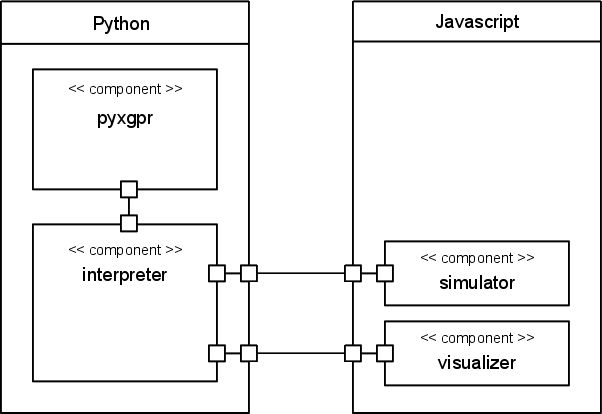
\includegraphics[width=0.7\textwidth]{solution/graphics/system-overview.png}
  \caption{Locates all cells within the boundary.}
  \label{fig:system-overview}
\end{figure}
\section{Implementation}
\subsection{Grids}
In the implementation, we introduced a concept called grid. A grid was a visual representation of an area (any area) divided into cells containing discrete values. The purpose of the grid was to easily view the actual situation and the predicted situation after reconstructing it based on samples from the actual situation (mobile phone sensor readings). As figure \ref{fig:grid-concept} shows, we used two separate grids placed next to each other where the left grid is always the actual situation and the right grid is always the predicted situation. These two grids served as a guide line throughout the implementation. If the grids did not look somewhat similar at all times, some error had been done. How these grids were used are explained in the following sections.

\begin{figure}[here]
\centering
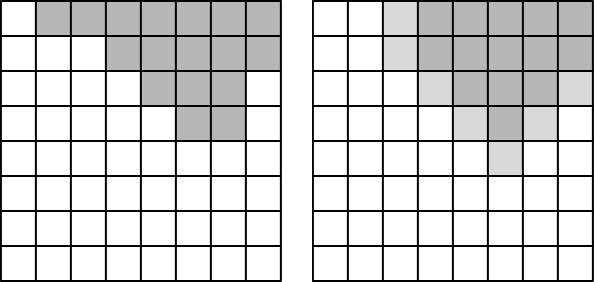
\includegraphics[width=0.5\textwidth]{solution/graphics/grid-concept.png}
\caption{Two grids are used to compare the actual situation on the left and the estimated situation on the right.}
\label{fig:grid-concept}
\end{figure}

\subsection{Simulating Data}
Simulating data was done in the left grid. At launch, the user had to choose a location for the initial fire. A user could start several fires at once, where each one would spread independent of the other fires. The spreading was done automatically for each time iteration.

The fire spread was implemented with a simple algorithm. Given a two-dimensional grid of cells, the more burning neighbours each cell C on the grid had, the higher the chances were for it to ignite. Because there is a maximum of eight neighbors, we divided the number of burning neighbors by the total number of neighbors as shown in figure \ref{fig:fire-probability}.

\begin{figure}[here]
\centering
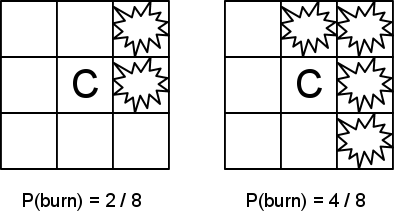
\includegraphics[width=0.5\textwidth]{solution/graphics/fire-probability.png}
\caption{Probability that fire will spread to a cell C on the grid without fire.}
\label{fig:fire-probability}
\end{figure}

The simple probability calculation was later extended to account for wind. Since wind can blow away smoke and heat, wind direction and magnitude directly affects how much impact each neighboring cell would have on C. To simulate this, each neighboring cell used a portion of the wind vector to produce a weight of impact. The sum of all these weights divided by a total weight became the new probability calculation in the fire spreading algorithm.

Humidity was implemented after wind. Humidity affects how fast fire spreads. It was implemented as a global value and had the same value for each cell. With this simplicity, we only had to either increase or decrease the total weight used in the probability calculation to adjust the rate of fire spread.

\subsection{Sensing Data}
After simulating data with wind and humidity, the next step was to use mobile phone sensors to read this data. Even if the current situation was known through the simulation at all times, we were only supposed to know the situation by the mobile phone sensor readings. To simulate sensing, two additional algorithms were used.

The first algorithm was a walking algorithm to simulate that people walk around with the mobile phone sensors. This algorithm assumed that sensors already had a position in order to do the following. For each time step, there was a fifty percent chance for each sensor to move. Because there were eight different directions to walk in a grid, the sensor picked a random direction. If the neighboring cell in the picked direction was on fire, the sensor had to pick another direction. In all, this algorithm only handled the location of the mobile phone sensors in the simulation. The next step after placing the sensors was to do readings.

The second algorithm was a sensing algorithm to provide known data used by the crisis mapping system. Because heat and smoke moves in the direction of the wind, the resulting sensor readings highly depended on wind and the location of the fire. Consider the example in figure \ref{fig:sense-concept}. Given the same wind vector W and two different neighbors at relative positions V1 and V2, each neighbor contributes differently to the sensor in C. In this particular case, the wind either blow heat and smoke away from C or into C depending on which neighbor it is.

\begin{figure}[here]
\centering
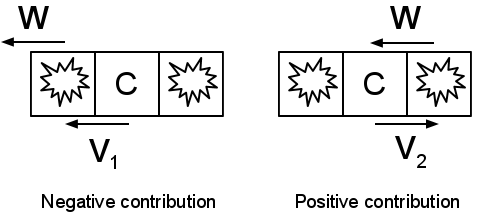
\includegraphics[width=0.65\textwidth]{solution/graphics/sense-concept.png}
\caption{Sensor readings are affected by wind and the positions of the neighboring emitting cells.}
\label{fig:sense-concept}
\end{figure}

The heat and smoke contribution to the sensor at C could be calculated as the sum of the cosine value of the angle between the wind vector W and the position vector for each neighbor. As shown in figure \ref{fig:sensor-contribution}, the cosine value could be divided into two ranges.

\begin{figure}[here]
\centering
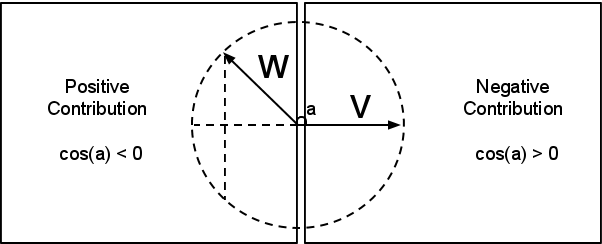
\includegraphics[width=0.65\textwidth]{solution/graphics/sensor-contribution.png}
\caption{Neighbor heat and smoke contribution is found by the cosine value between on wind W and neighbor position V relative to the sensor.}
\label{fig:sensor-contribution}
\end{figure}

The range [-1,0] was equal to positive contribution while the remaining [0,1] was equal to negative contribution. In case of a negative contribution, the contribution can simply be treated as 0 because heat and smoke would blow away from the sensor. To further simplify, by taking the absolute value of the positive contribution range [-1,0], the new range became [0,1] where 0 is the lowest and 1 is the highest contribution. This could be used as a coefficient to the heat and smoke emitted by this neighbor. Given that there are eight neighbors each indexed by i, the resulting mathematical formula used in the sensing algorithm is as follows:

\[
  c = \sum_{\substack i=1}^8\left\{
  \begin{array}{l l}
    |V_i \cdot W / \left(|V_i | \cdot |W| \right)| & \quad \text{if $V_i \cdot W < 0$}\\
   0 & \quad \text{if $V_i \cdot W >= 0$}\\
  \end{array} \right.
\]

\section{Fire Interpreter}
The fire interpreter's job is to receive input from the simulator and 
calculate values for the received cells. The calculated values are then posted to the visualizer. The advanced regression calculations are done by the library pyXGPR. This is a Gaussian Process Regression library implemented with Python. It produces a mean and a variance when used correctly. The first input parameter \textbf{X} is a list of points which tells where the training data is located. Another parameter \textbf{Y} contains the values to the training data. The last interpreter generated parameter \textbf{x star} contains the points where we want to find the mean and the variance. In addition to these parameters the library needs to be told what covariance functions pyXGPR should use to calculate the correlation between the cells in \textbf{X}, \textbf{Y} and \textbf{x star}. There is also added parameter values to these functions.
\\\\
The most basic use of pyXGPR is one dimensional (line regression) where \textbf{X} is the location and \textbf{Y} is the value. The fire interpreter uses regression in three dimensions where \textbf{x} and \textbf{y} are the map coordinates and an additional parameter \textbf{t} is for time. \textbf{t} is necessary to save earlier sensor data which later are utilized in predictions. It should also be mentioned that before this implementation, this was done by saving the best data. Best data is to be understood as the data which has the lowest variance. Data with lower variance would be applied to the saved map. This hack and the implementation of t is done because previous sensor data is important as long as they are weighted less than the newest sensor data. As time increases there will be sensor data covering a larger portion of the map, but the old sensor data will have less weight and thus giving new sensor data the opportunity to be taken into account. Figure \ref{fig:timeElapse} illustrates this.
\begin{figure}[here]
  \centering
      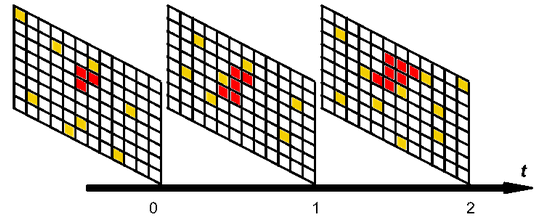
\includegraphics[width=0.5\textwidth]{solution/graphics/timeElapse.png}
  \caption{The fire interpreter saves the sensor data (yellow dots) and gives them a timestamp \textbf{t}. Earlier data is weighted less since the current \textbf{x star} and \textbf{X} has the same and last value for \textbf{t}. }
  \label{fig:timeElapse}
\end{figure}
\subsection{Performance}
The simulation map is 71 X 71 squares. GPR calculates the correlation between all points. This means pyXGPR creates huge matrices. As \textbf{t} increases the matrices grow larger and thus the execution time rises. The first version of the program used more than 6 minutes to run on a normal laptop. To better the performance it was found necessary to locate some squares which did not need to be calculated. Cells containing sensors was therefore removed from \textbf{x star} since the values were already there. With the introduction of \textbf{t}, the matrices became larger and execution time rose and once again it was necessary to find some steps to improve the performance. For a cell to be added to \textbf{x star} it had to be close to sensor which communicated fire. This was done by finding the euclidean distance between all cells which had no value and all sensors which communicated fire. This reduced the number of points in \textbf{x star} significantly. As time increases Another measure taken to reduce the execution time was to save cells which was calculated to be on fire. From these the euclidean distance to all points were calculated and if they were within a certain distance they would be added to \textbf{x star}.
\\\\
Before the interpreter posts the calculated data to the visualizer it converts the mean values to discrete values which is used in the visualizer to decide how intence the fire is burning. A threshold to determine if there should be fire is set, but can be difficult to determine as time progresses. The input values for sensors sensing fire is $0 $ to $10$, while sensors which are not sensing fire is converted from $ 0 $ to $ -1 $. The reason for the conversion is to get some more distance between fire and not fire. The fire threshold is set low to make sure all the realistic fire is covered.
\\\\
\subsection{Changes in pyXGPR kernel to support wind}
The simulation use wind as a crucial parameter to decide where the fire is spreading. Wind is therefore clever to use in the interpretation process. To make it a useful parameter the kernel in pyXGPR has been edited. The kernel contains all the different covariance functions and noise functions. The modification has been done in the function which measures the squared distance between two points. The squared distance is measured by creating two matrices for each dimension. In the fire interpreter these dimensions are \textbf{x}, \textbf{y} and \textbf{t}. One matrix containing all sensor data is deducted from a matrix containing all the uncalculated data. The dimensional result is multiplied with itself and added to a distance matrix. All dimensional results are added to the distance matrix. 
\\\\
\begin{eqnarray}
\theta = cos^{-1}\left(\dfrac{vector_{ij} \times windVector}{\|vector_{ij}\| \times \|windVector\| } \right) 
\label{eq:int-angle}
\end{eqnarray}
\begin{eqnarray}
weight = \dfrac{\theta}{\pi}
\label{eq:weight}
\end{eqnarray}
\begin{eqnarray}
\begin{bmatrix} distance_{11} & distance_{1j} \\ distance_{i1} & distance_{ij} \end{bmatrix} \times 
\begin{bmatrix} weight_{11} & weight_{1j} \\ weight_{i1} & weight_{ij} \end{bmatrix}
\label{eq:hadamard}
\end{eqnarray}
\\\\
Before these calculations the interpreter implementations in this function creates a weight matrix which has the same column and row values as the distance matrix. This weight is calculated with the forumula in \ref{eq:weight}. The Hadamard\cite{hadamard} product (see equation \ref{eq:hadamard}) of these two matrices is returned as the new distance matrix. 
\\\\
Where $ vector_{ij} $ is the vector from sensor position $i$ to uncalculated position $j$. The weight is further normalized to better fit the wind. If $ vector_{ij} $ is between $ 90^{\circ} $ and $ 180^{\circ} $ the weight will be normalized to larger than one and less than one if the angle is less than $ 45^{\circ} $. The values in the weight matrix is multiplied with the values in the distance matrix to create a hadamard\cite{hadamard} product. $ vector_{ij} $ in the weight matrix is multiplied with $ vector_{ij} $ in the distance matrix. This modifies the distance matrix where some values are reduced and some are increased, determined by their vector direction. The correlation of cells looks at the distance between them. Therefore decreased distance to a sensor sensing fire gives a cell a higher probability of being on fire. Sensors which does not detect fire will have a weight of one.
\subsection{Unexpected predictions with wind}
\label{wind-problem}
\begin{figure}[here]
  \centering
      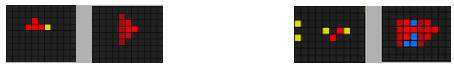
\includegraphics[width=1.0\textwidth]{solution/graphics/wind-problem.png}
  \caption{The left image illustrates when wind is used in predicting fire, while the right image illustrates the faults with a pure wind implementation. The blue dots are where the there should have been predicted fire.}
  \label{fig:wind-problem}
\end{figure}
The implementation of wind is working, but has some drawbacks. The first image in figure \ref{fig:wind-problem} illustrates how the fire is predicted when the wind is blowing from the east. The spread starts where the sensor is located and continuous in the shape of a triangle towards west. This looks good in the first image, but the second image illustrates the drawbacks. The wind is still blowing from the east and the two sensors detecting fire are on a horizontal line. The right tips of the predicted fire is where the sensors are located. The blue squares is used to highlight where there should have been predicted fire. This situation occurs because the blue squares are closest to the second sensor. The vector which goes from the second sensor to the any of blue square has an angle which is more than $ 45^{\circ} $ when compared to the wind vector which is $ \left[-1,0\right] $. Problems with predicting the middle part of the fire can occur when the the size of the predicted fire is becoming quite large. To solve both these problems there has been developed two solutions which have been tested with varying results. The first solution looks at the correlation between all sensors sensing fire while the second solution uses some techniques found in graphical programming. Another approach to these problems would be to use dynamic parameters. As the fire progressed the parameters would change in accordance to the size of the fire. But problems arises with such a solution as well. The edge of the fire would be more likely to be smudged out and it would in some cases predict fire in areas where there were no fire.
\subsubsection{Solution 1 to unexpected predictions with wind}
Burning sensor correlation was one approach to solve the problem when applying wind. It creates a list of all sensors which are sensing fire. Each element in the list has vectors to all other sensors communicating fire. In figure \ref{fig:burning-sensor-correlation} the green triangle is an uncalculated point while the numbered red circles are sensors sensing fire. There are vectors from sensor 1 to all other sensors sensing fire and a vector to the green triangle. This is an illustration of one of the entries in this list. The basis for this theory is that there is probably actual fire between the sensors. The blue vector compares direction with all the black vectors, see \ref{eq:int-angle}. It finds the black vector which has the most similar direction and check if it is within a certain threshold. If this comes out positive the distance for this point to sensor one will be multiplied with a number less than one, else it would be multiplied with one.
\begin{figure}[here]
  \centering
      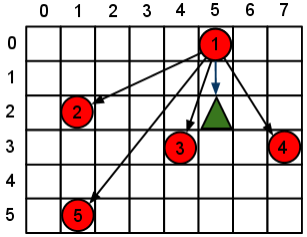
\includegraphics[width=0.4\textwidth]{solution/graphics/burning-sensor-correlation.png}
  \caption{All sensors (red) are sensing fire and sensor one has a vector to all other vectors sensing fire. The green triangle is an uncalculated point. Burning sensor correlation looks for the black vector which has the most similar angle to the closest blue vector.}
  \label{fig:burning-sensor-correlation}
\end{figure}
This approach has a fault. When a situation like \ref{fig:wind-problem} (second image) occurs it would predict fire against the wind. The burning sensor correlation would neutralize the added wind to such a degree that it was removed. The complexity with this solution is high and thus the execution time rises fast as \textbf{t} increases and the fire interpreter uses more data. As this solution was developed it would handle multiple fires badly.
\subsubsection{Solution 2 to unexpected predictions with wind}
In the second approach to solve the wind and filling issues, components from computer graphics were used. The outer boundary of the sensors sensing fire was chosen. The shape will be a convex polygon. Uncalculated cells within this polygon will have a higher probability of being on fire in the prediction. As in the burning sensor correlation implementation it is assumed its a higher probability of being fire between sensors sensing fire.
\begin{figure}[here]
  \centering
      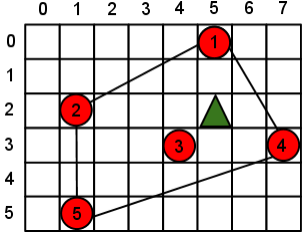
\includegraphics[width=0.4\textwidth]{solution/graphics/graphical-boundary.png}
  \caption{Locates all cells within the boundary.}
  \label{fig:graphical-boundary}
\end{figure}
To locate all the outer cells Graham's scan \cite{graham} was applied. When these points were found Bresenham's\cite{bresenham} line algorithm was used to find the in between cells. The result was all cells which the lines covered in figure \ref{fig:graphical-boundary} was retrieved. After this a scan line fill algorithm was used to find all the cells within the polygon. These steps resulted in a list of cell positions. This list was used when calculating the wind in accordance to wind direction. If the cell to be evaluated was inside this polygon the weight was multiplied with a number lower than one. This solution is also much faster than the first one. The Graham's scan and Bresenham's line algorithm was used as third party code, meaning we did not implement them. But the scan line algorithm was implemented in the kernel. Currently it does not handle multiple fires. If the two fires started at different \textbf{t} it could be possible to walk on predicted fire from one sensor to all the others.

%\include{./performance/performance}
%\chapter{Discussion}
\section{Results}
The results are divided into two groups, simple simulation and advanced simulation. The results addressed in this section are reasonably representative for the average results.
\subsection{Results with simple simulation}
The simple simulation is characterized by sensors being spread relatively even throughout the map. The rule is that a sensor cannot touch another sensor. When using the simple simulator each sensor can only sense its closest neighbours. 
\\\\
Figure \ref{fig:simple-results1} illustrates the success of the fire interpreter. The light green color is where the actual fire is and where the interpreter predicted it to be. Therefore the color of success. The dark green color is area where the interpreter thought it would be fire, but was not. The red parts are the actual fire which the interpreter did not predict. 
\begin{figure}[here]
  \centering
      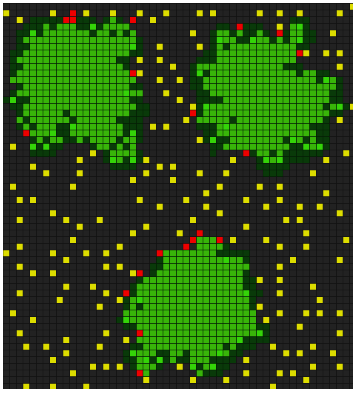
\includegraphics[width=0.7\textwidth]{discussion/graphics/results-simple-compare.png}
  \caption{The intense green is where the fire interpreter predicted correctly. The dark green is where the fire interpreter thought it was fire, but it was not. Red dots are where there actually was fire, but the predictor was unable to predict it.}
  \label{fig:simple-results1}
\end{figure}
\subsection{Results with advanced simulation}
The advanced simulation mimics the effect of humidity and wind has on a fire. The sensors are spread more randomly than in the simple simulation. They can also sense with a larger range. The default is two cells. The fire interpreter used the wind add-on in the kernel in the successful tests, while it was turned off in the tests which did not have too good results. There are a number of parameters which has been tweaked to get good results. These different parameters makes it more difficult to get an accurate prediction. Figure \ref{fig:wind-advanced-bresenham-large} illustrates the predicted fire on top of the actual fire when the wind is blowing from west.  
\begin{figure}[here]
  \centering
      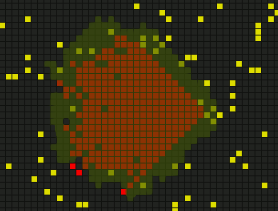
\includegraphics[width=0.5\textwidth]{discussion/graphics/wind-advanced-bresenham-large.png}
  \caption{The dark green overlay is where the fire interpreter predicted the fire to be. The red covered by the green overlay is where the fire interpreter predicted correctly and the red dots without any overlay is where there was fire, but did not predict.}
  \label{fig:wind-advanced-bresenham-large}
\end{figure}
The prediction is covering a larger area than the actual fire. This is because the sensors are sensing 2 cells away. In figure \ref{fig:wind-advanced-bresenham-large} this can be observed with the right most predicted fire. The two sensors which lays beneath the right most predicted area is sensing fire and therefore the prediction is set from this point. The first cells north and south of this area has also been calculated to be on fire. This is because of Bresenham’s line algorithm which interprets these two cells to be on the outer boundary of the sensors sensing fire. The algorithms from computer graphics is used to make sure there are no holes inside the predicted fire and to prevent wind problem (chapter \ref{wind-problem}).
\begin{figure}[here]
  \centering
      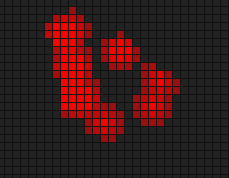
\includegraphics[width=0.5\textwidth]{discussion/graphics/advanced-without-wind-and-bresenham.png}
  \caption{Wind and graphical algorithms disabled in the advanced simulation creates holes and shows a lack wind direction.}
  \label{fig:advanced-without-wind-and-bresenham}
\end{figure}
\\\\
Figure \ref{fig:advanced-without-wind-and-bresenham} illustrates what is happening when wind and the graphical algorithms are disabled. Within the domain of the advanced simulation the results achieved with wind and the graphical algorithms. The prediction with this set up reproduces the shape of the actual fire with a satisfactory result. The area of the shape is larger than the actual fire. The philosophy was always to air on the side of safety. Meaning that the fire interpreter aimed to detect all fires and as such a few false positives were deemed to be acceptable.
\section {Practical Issues}
There are several practical issues that arises if this system should be put into motion. Collecting sensor data from a mobile phone and sending it to the crisis mapping system creates huge security and privacy issues. Personal data, like location and private conversations, may be useful in mapping a crisis, nevertheless the program should endeavour to protect the user and not disclose any information that is not relevant. In addition, the collected data should be transferred as fast as possible, over a secure connection, from the phone to the crisis mapping system to allow the program to react to new sensor readings as quickly as possible.

The system will always rely on sensors and people carrying a mobile phone capable of sensing. People will spectate on fires, but they will do it outside range of the heat and smoke. If it is blowing in one direction, the smoke and heat will drive people away from one side of the fire, meaning that there will not be sensor readings around the fire after they have moved away.

The mobile phone sensing scheme as with most other schemes, there are limitations to what is possible to achieve. Firstly, the crisis mapping system cannot account for human behavior. When a fire crisis occurs, people need to have a mobile phone with sensors available at that time, and people need to keep the mobile phone sensors close to the crisis situation. The further away the reading is made from the fire, the lower heat and smoke intensity would be read. Even if people would spectate the fire, they would do so away from harmful intensity. In all, this means that there is less good data to work with.
%\chapter{Conclusion}
\chapter{Introduction}

\section{Background}

Crisis Mapping is the process of collecting, analyzing and visualizing crisis data for further crisis management. The goal is to provide better real time decision support to determine the best course of action in a changing or evolving crisis environment. This in turn provide help to crisis victims and save more lives.

In 2010, a major earthquake crisis struck Haiti. The shock measured 7.0 on the moment magnitude scale (MMS) and was followed by another 52 aftershocks of 4.0 MMS or higher over 12 days. 1 517 000 people and their dependents were affected. People were in need of housing, food and medical attention. Mapping these needs would improve further crisis management \cite{}.

The needs on Haiti were mapped by Ushahidi, an open source software. This software collects, analyzes and visualizes data from social media, text messages and more. The Haiti government took advantage of this software and allowed crisis victims and bystanders to report needs to temporary web services and text message services. These services together with Ushahidi provided a crisis map that aided the government to send help where it was needed \cite{}.

Today, researchers are investigating how to use mobile phone sensors to map crisis situations. Many mobile phones have built-in sensors such as microphones, accelerometers, gyroscopes, barometers and GPS. In theory, these sensors can be used to detect earthquakes, fires, explosions, collisions and other crisis situations by reading abnormal magnitudes or patterns in sound, acceleration, air pressure and temperature. Mobile phones can be used to report this abnormality to a central crisis mapping system and possibly aid further crisis management.

\section{Problem Statement}

CISTECH of the University of Agder proposed a basic project about crisis mapping using mobile phones. Because crisis mapping is a general term and includes a broad range of different crisis situations, we had to narrow down the goal of the project. After consulting with our supervisor, the final goal was to create a prototype crisis mapping system that could detect fire using mobile phone sensors. We chose fire in specific because it can change or evolve over time. However, the chosen topic does not come without a set of practical limitations.

Given the project goal, we focused on two main problems that had to be solved. Firstly, fires had to be simulated. There was no way to justify starting real fires to gather this data. Simulating fire is challenging because fire spreads based several factors such as wind, heat, humidity and other over time. Secondly, mobile phone sensors do only report readings at their location and do not cover burning areas without nearby sensors. Uncovered areas have to be guesstimated.

\section{Literature Review}

\subsection{A Survey of Mobile Phone Sensing}

The field of mobile phone sensing is rapidly expanding. The accelerometer in a smart phone can determine whether the user is walking, running or standing still. The microphone can collect audio. The light sensors can determine whether the phone is in a pocket or not and the barometer can determine air pressure. In addition data can be combined from different sensors to make assumptions, for instance a phone can sense that a user is walking down a hill and in which direction he is going. Specialized sensors have also been used to measure air pollution and could perhaps be used to detect explosive residue.

There are many issues with properly utilizing and gathering data. First of all a large amount of users to properly test a system is needed. This can be solved by distributing the application via the App stores and providing an incentive for the users to use it. Second there are huge privacy issues with listening in on private conversations using the microphone and tracking the user via the GPS. This can somewhat be fixed by calculating any result on the phone and sending only the results, however this would require more resources from the phone and would likely limit battery time or performance. Some studies have shown that sensing systems have reduced the standby time by significant amounts, vastly affecting the user experience.

Creating a system that produce accurate results may also be slightly problematic as vendors did not foresee the use of their sensors in new applications. The sensor sampling rate varies based on the CPU load and the API and OS does not support complete access to the sensors. However, as the mobile phone sensing field is growing vendors are likely to catch on and provide better sensors and sensor support in future releases.

Moreover, it is also difficult to create a program that fully accounts for all possible instances. Explosives used in demolition and terrorism both create the same or similar sound and gun fire while hunting sounds the same as gun fire in a super marked. A phone also needs to know if it is currently inside a container where the sound might be suppressed, in which case the system might become more sensitive to sound. This in turn can be somewhat solved by using light or proximity sensors however there might be cases where the phone is placed in an unusual location and therefore provides inaccurate results.

\subsection{Distributed Perception Networks for Crisis Management}

Distributed Perception Networks for Crisis management (2006) focuses on the fusion of information gathered from fixed sensors and human perception. The fixed sensors are few and scarcely distributed in an area where a crisis could have devastating consequences. Endsley’s model tells that first comes perception, then comprehension and projection. The paper focuses on combining the perception of humans and the fixed sensors to create a clear picture of the situation. For example when the sensors are picking up dangerous levels of ammonia in the air the system will use human perception to gather more input. This is done by sending SMS to everyone in that area where the query could be; “Do you smell ammonia?”. By using human perception the crisis management team will get a richer and more detailed map instead of only using the scarcely distributed fixed sensors.

Sensor readings and public perception results in a vast amount of information which needs to be processed. Since it is such an enormous task for manual human labour the paper proposes to use a Bayesian network to find the most probable cause of the crisis. There is a large degree of uncertainty when gathering huge amounts of information from people and possibly faulty sensors. The DPN architechture represents a multi agent system which means it can comprehend large problems in efficient manner. A set of nodes is processed by one agent before they send it to their father node. The paper does not suggest how to calculate how toxic the air will become where it will spread.  

\subsection{Video about how crisis mapping helped during the Haiti earthquake}

When the earthquake hit Haiti in 2010, there was an initiative to map where help was needed to increase the efficiency of rescue personnel. In addition, no emergency call centers were operational directly after the earthquake, further increasing the value of a crisis map in this particular situation. People in need of help would send a text message signifying their location and situation, operators would then note what help was needed and place the note on the map showing the location. Organisations could then use this map to deploy personnel in areas where they were needed the most. In addition, any volunteers could view the map and help if they were able.

One thing to note about this system was that messages were written in different languages and then translated to English. Most of the translation were done with assistance from the general public, this highlighted the positives of a crisis mapping system that is open to the public.

By using a map and plot what is happening in the different areas, organisations that are trying to help may send their resources to the correct locations at the right time. Organisations may also inform people where dangerous locations are during the crisis and guide the people in that area to a safe location. In addition, they may plan their next move as they observe the evolving crisis. People that also are able to see this crisis map may see the locations that are dangerous, for example they can then use the map to spot a burning building and head in a different direction. 

\subsection{A Real-time Disaster Situation Mapping System for University Campuses}

A real-time disaster situation mapping (RDSM) system is a web-based system which acts as a social media. The system helps its users and the disaster management team during a crisis situation by giving the disaster management team a clear overview of the situation and the users can use the system to acquire their location and the nearest exit.

The RDSM system is based on some conditions such as disaster type, place of use and targeted users. The main focus of the system is to protect people during and immediately after a disaster based on the assumptions that the earthquake has a minimal impact on the university buildings. In the event that the university buildings are severely damaged then important equipment such as servers, Wireless LAN, etc. may be out of commission and the system may end up not working properly. The mobile devices, such as computers or phones, are assumed to be in use and connected to the servers during the disaster situation. The RDSM system can be accessed inside the university as well as in the evacuation office by any employee with sufficiently high authority level.

The RDSM system has  two major  parts, called situation gathering sub system (SGS) and the situation mapping sub system (SMS) \cite{}. The SGS allows people in the campus to send situation information about their location, such as degree of longitude, latitude and name of the place at the time of the disaster, using their mobile devices.The location information can be identified by manual entry as well as by the automatic acquisition using Place Engine. Place Engine is a service where users can send location information, even though they do not recognize their locations, by utilizing Wi-Fi devices. Some requirements have to be satisfied in order to set up the Place Engine for automatic data acquisition of location information. First, the Wireless LAN access point data must be saved in the Place Engine database. Secondly, at least one access point must be reachable from the users  location. Next, access to the Place Engine server must be feasible. Finally,  the users’ mobile device(s) (PC or phone) must be equipped with Wireless LAN (Wi-Fi) equipment and the client software must be installed on those mobile device(s) \cite{}. The users can send situation information from the situation data entry screen by accessing the SGS. Speech to text transformation is achieved by using “w3voice”, which is a development kit for voice-enabled web applications \cite{}. Therefore the informers can send voice data, text data as well as video via the disaster situation entry screen.The entered situation data is stored in the situation database. 

The SMS reads data from the situation data base updated by SGS and it will replicate that data onto maps sent by the users. The more detailed information of the disaster situation is shown by the time series on the map screen. The users can also access the voice or image data  in order to get a clear and accurate information about the crisis situation.Situation data that are described by text data are rendered on this “png” map in SMS. In order to show the disaster affected areas (points) on the map, Google maps are used to get the degrees of latitude and longitude of two different points. “By calculating the distance between user’s location and the point obtained from Google maps, users’ location is identified from the reduced scale distance that is started from two different points” \cite{}.

\section{Solution Approach}

In this project, we simulated our crisis mapping system using two grids. Both grids represented the same area (any area) divided into equally sized squared cells. In the first grid, we let fire and mobile phone sensors spread freely over the cells. In the second grid, we estimated the fire situation based on mobile sensor readings from the first grid using Gaussian Processes Regression (GPR). Having the actual situation put next to the estimated situation, we could easily verify the strength and weaknesses of both the crisis mapping system and concept in terms of similarity and differences.

\section{Report Outline}

Chapter one introduces crisis mapping, what problem this project is trying to solve and the solution approach. In addition the chapter contains literature reviews of relevant papers. The second chapter of the report contains the theoretical background which the project is based on. The fire theory is used in the implementation of the fire simulation and the theory on Gaussian Processes is used in the implementation of the interpreter.

Chapter tree describes the project requirements and limitations. Additionally it outlines what the simulation and interpreter were expected to do, how the expected functions were implemented and if our way of implementing the features were the correct one. The fourth chapter contains the discussion which aims to present the results, explain why the solution approach was chosen over other alternative solutions and how well the solution satisfied the requirements.

Finally, chapter five contains the conclusion. It endeavours to determine whether the results makes a difference to existing solutions and what the benefits are for system users. Additionally it contains proposed next steps if the project were to be continued.
\chapter{Theory}
\section{Gaussian Processes for Regression}
Mathematical solutions such as linear regression are often used to predict unknown values based on similar values. Depending on input data, output accuracy and simplicity, mathematicians are encouraged to use several other methods as well.
Gaussian Process Regression (GPR) is one of the popular methods has been used due to several reasons such as:
\begin{itemize}
\item Very accurate output
\item Less number of variables
\item Learning by experience
\end{itemize}
Correct predictions must be based on the correct assumptions. Even though GPR is  learning from experience, it is not “free form” which means it is not automatically generated[ ]. Other techniques, such as “squared exponential”, can be used when the users are unable to do even basic assumptions.
\\\\
It is acceptable to assume that each observation point has data distribution similar to normal distribution. Therefore, it is needed  to calculate the mean value and variance for all predictions.
\begin{figure}[here]
  \centering
      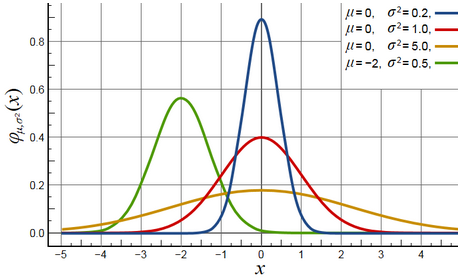
\includegraphics[width=0.9\textwidth]{theory/graphics/normal-distribution.png}
  \caption{Normal Distribution curves\cite{normal-dist}. }
  \label{fig:normal-distribution}
\end{figure}
\subsection{Covariance Function}
In general, users can assume that “partner GP’s mean is zero” everywhere\cite{simple-covariance}. Therefore, two similar cases are related to each other by a covariance function $ k(x-x') $. Among the various options “squared exponential” is one of the popular choices for the covariance function.
\begin{equation}
k(x,x^{'})=\sigma_{f}^{2}exp\left[ \dfrac{-(x-x^{'})^{2}}{2l^{2}} \right]
\label{eq:simple-covariance}
\end{equation}
\begin{eqnarray}
 x - x^{'} &=& Distance\hspace{7pt} between\hspace{7pt} observation\hspace{7pt} data    \nonumber \\
  l &=& length\hspace{7pt} parameter \nonumber \\
  \sigma_{f}^{2} &=& Maximum\hspace{7pt} allowable\hspace{7pt} covariance
\end{eqnarray}
To predict accurate data for a smooth curve, input (or observed) data from the neighbors must be identical. By studying the above equation, we can understand that $ \sigma_{f}^{2} $ is increased for functions which cover a wide area through the y-axis. When the $ (x-x') $value becomes larger, $k(x-x')$ approaches zero depending on the length of parameter $ l $.
\\\\
The effects of the length parameter $l$, can be explained as follows: Lets assume $l=0.1$ for a particular prediction and graph  $f(x)VS x$, which is shown in figure \ref{fig:length-parameter}. It is clear that the curves are not aligned\cite{intro-to-gpr}.
\begin{figure}[here]
  \centering
      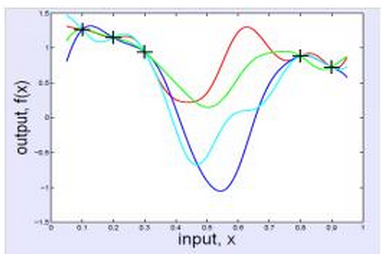
\includegraphics[width=0.65\textwidth]{theory/graphics/effects-of-l.png}
  \caption{When $l = 0.1$. \cite{length-parameter}. }
  \label{fig:length-parameter}
\end{figure}
So, we change $l=0.3$ and evaluate the results. This is shown in figure \ref{fig:length-parameter-03}. It is clear that the curves are more aligned here than in figure \ref{fig:length-parameter}.
\begin{figure}[here]
  \centering
      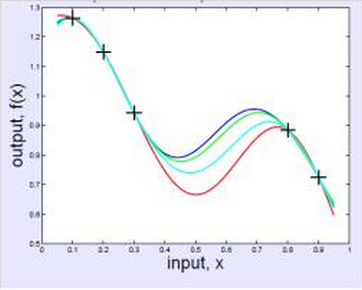
\includegraphics[width=0.65\textwidth]{theory/graphics/effects-of-l-03.png}
  \caption{When $l = 0.3$. \cite{length-parameter}. }
  \label{fig:length-parameter-03}
\end{figure}
Since the curves are not perfectly aligned, length parameter l, is increased further and result is evaluated. In figure \ref{fig:length-parameter-05} we set $l=0.5$ and evaluate the results. Here we can observe that the curves are perfectly aligned \cite{length-parameter}.
\begin{figure}[here]
  \centering
      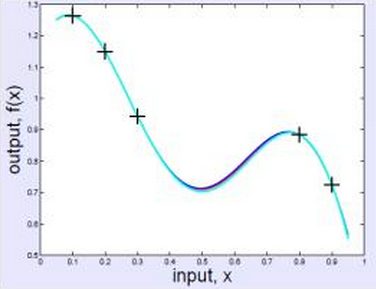
\includegraphics[width=0.65\textwidth]{theory/graphics/effects-of-l-05.png}
  \caption{When $l = 0.5$. \cite{length-parameter}. }
  \label{fig:length-parameter-05}
\end{figure}
Apart from this, function consists of additional part to represent errors. This is an important part, when GPR is used to predict practical events. (e.g. environment temperature can be vary, due to external factors such as wind ).
\begin{equation}
k(x,x^{'})=\sigma_{f}^{2}exp\left[ \dfrac{-(x-x^{'})^{2}}{2l^{2}} \right] + \sigma_{n}^{2}\delta(x,x^{'})
\label{eq:referanceName}
\end{equation}
However, people preferred to keep $ \sigma_{n}^{2} $ separately and work on covariance and error to simplify the calculation.

\subsection{Method of Calculation}
The covariance value, $ k(x,x') $ can be calculated with each observed data in respect to each other observations. Values can be represented by a metric. By assuming that five observations have been conducted, $ x1, x2, x3, x4, x5 $. $k(x,x')$ value for those observations can be written as follows:
\begin{eqnarray}
K = 
\begin{bmatrix} 
k(x_{1}x_{1}) & k(x_{1}x_{2} & k(x_{1}x_{3} & k(x_{1}x_{4} & k(x_{1}x_{5} \\ k(x_{2}x_{1}) & k(x_{2}x_{2} & k(x_{2}x_{3} & k(x_{2}x_{4} & k(x_{2}x_{5} \\
k(x_{3}x_{1}) & k(x_{3}x_{2} & k(x_{3}x_{3} & k(x_{3}x_{4} & k(x_{3}x_{5} \\ k(x_{4}x_{1}) & k(x_{4}x_{2} & k(x_{4}x_{3} & k(x_{4}x_{4} & k(x_{4}x_{5} \\
k(x_{5}x_{1}) & k(x_{5}x_{2} & k(x_{5}x_{3} & k(x_{5}x_{4} & k(x_{5}x_{5} \\ \end{bmatrix}
\label{eq:k-matrix}
\end{eqnarray}

This is a symmetric metric, $k(x1,x2)$ and $k(x2,x1)$  where both elements have the same values. All diagonal elements are equal and show the highest $k(x,x')$ value since $ \dfrac{-(x-x^{'})^{2}}{2l^{2}} $  becomes zero.
\\\\
When the position is moving away from the diagonal line of the matrix, the value of $k(x_{n},x_{m})$ goes towards zero. In other words, if the matrix contain higher number of rows and columns, the values of positions such as far away from the diagonal are almost equal to zero, while diagonal values shows maximum covariance value.
\\\\
While the $K$ matrix gives the covariance values for observed data points the $K*$ matrix gives the covariance values for considered points compared to other observed points. Let’s make the matrix $K_{*}$ relative to the above five positions.
\begin{equation}
K_{*} = [k(x_{*},x_{1}) \hspace{10pt} k(x_{*},x_{2}) \hspace{10pt} k(x_{*},x_{3}) \hspace{10pt} k(x_{*},x_{4}) \hspace{10pt} k(x_{*},x_{5})]
\label{eq:referanceName}
\end{equation}
$K_{**}= k(x_{*} x_{*})$ also can be found same way as it is directly given by $k(x,x')=\sigma_{f}^{2}$. From the above values, mean and variance values for a given $y_{*}$ can be found in the following way:
\begin{eqnarray}
 \overline{y_{*}} &=& K_{*}K^{-1} y    \nonumber \\
 var(y_{*})&=& K_{*}_{*}K_{*}K^{-1}K_{*}^{T}
\end{eqnarray}
\begin{eqnarray}
y = 
\begin{bmatrix} 
y_{1} \\ y_{2} \\ y_{3} \\ y_{4} \\ y_{5} \\ \end{bmatrix}
\label{eq:k-matrix}
\end{eqnarray}
When finding the variance, a suitable confidence level must be selected according to the prediction (e.g. 95\% confidence level).
\subsection{Prediction of  Temperature Using Gaussian Process Regression}
The objective is to predict temperature at a particular point by interpreting other observed data. Imagine the following situation: The area highlighted in gray colour has sensors (Thermometer) to observe the temperature and one would want  to predict the temperature on red colour(3,3) in figure \ref{fig:value-matrix}.
\begin{figure}[here]
  \centering
      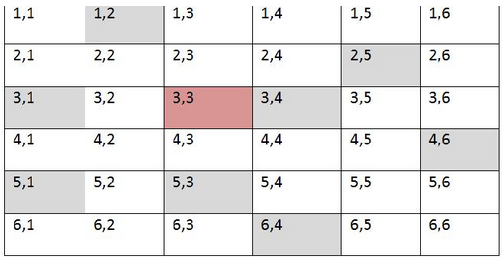
\includegraphics[width=0.65\textwidth]{theory/graphics/value-matrix.png}
  \caption{ Value matrix. }
  \label{fig:value-matrix}
\end{figure}
Since we can find the distance between each cells, it is possible to define a covariance function using observed data (given from thermometers). $ \sigma_{f}^{2} $ and $ l $ (length parameter) can be determined by using the observed data. Thereafter, $ K_{**} $, $ K_{*} $, $ K $ matrices can be determined. This will give the values for mean and variance. Finally, it is possible to plot the graph and this will give the predicted values for any positions within the considered area.

\chapter{Solution}
\section{Requirements}
The requirements in this project could be derived from the very definition of crisis mapping: collect, interpret and visualize crisis data.

Data need to be collected by mobile phone sensors readings. It can be representative, meaning that it does not need to be real world values. Nevertheless, it should be possible to distinguish between high and low values and the physics still needs to be real. This way, it is not necessary to start real fires to obtain some real data. It is adequate to simulate the data in order to prove or disprove that the crisis mapping using mobile phone sensors work. However, there are conclusions that can not be drawn solely by individual sensor readings.

Sensor readings can and need to be interpreted on a collective basis in order to get more data out of the related crisis situation. The interpretation should be able to estimate the actual situation based on a limited number of sensors. This is due to the fact that there is no way to guarantee that there are adequate number of sensors available at the crisis location at any time. After the interpretation, the collected data and the data provided by the interpretation are still not humanly readable and therefore needs to be visualized.

The interpreted situation needs to be visualized so that crisis management teams could use it to make better decisions. It is adequate that the estimated values can be read and compared with the actual values to visually determine the performance of the system.
\section{Design}
In the implementation, we introduced a concept called grid. A grid was a visual representation of an area (any area) divided into discrete valued cells. The purpose of the grid was to easily view the actual situation and the predicted situation after reconstructing it based on samples from the actual situation (mobile phone sensor readings). As figure \ref{fig:system-overview} shows, we used two separate grids placed next to each other where the left grid is always the actual situation and the right grid is always the predicted situation.
\begin{figure}[here]
  \centering
      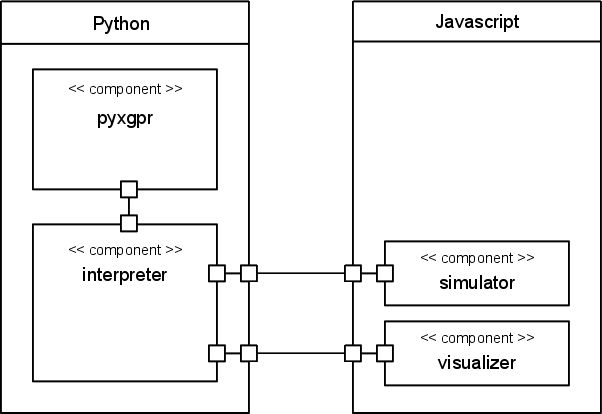
\includegraphics[width=0.7\textwidth]{solution/graphics/system-overview.png}
  \caption{Locates all cells within the boundary.}
  \label{fig:system-overview}
\end{figure}
\section{Implementation}
\subsection{Grids}
In the implementation, we introduced a concept called grid. A grid was a visual representation of an area (any area) divided into cells containing discrete values. The purpose of the grid was to easily view the actual situation and the predicted situation after reconstructing it based on samples from the actual situation (mobile phone sensor readings). As figure \ref{fig:grid-concept} shows, we used two separate grids placed next to each other where the left grid is always the actual situation and the right grid is always the predicted situation. These two grids served as a guide line throughout the implementation. If the grids did not look somewhat similar at all times, some error had been done. How these grids were used are explained in the following sections.

\begin{figure}[here]
\centering
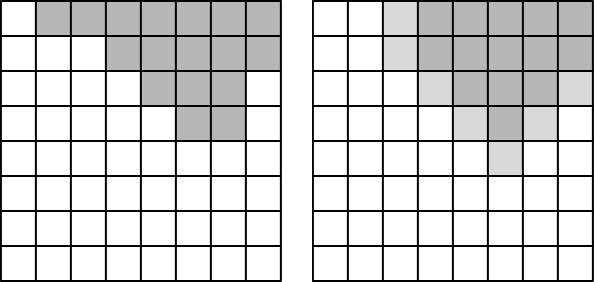
\includegraphics[width=0.5\textwidth]{solution/graphics/grid-concept.png}
\caption{Two grids are used to compare the actual situation on the left and the estimated situation on the right.}
\label{fig:grid-concept}
\end{figure}

\subsection{Simulating Data}
Simulating data was done in the left grid. At launch, the user had to choose a location for the initial fire. A user could start several fires at once, where each one would spread independent of the other fires. The spreading was done automatically for each time iteration.

The fire spread was implemented with a simple algorithm. Given a two-dimensional grid of cells, the more burning neighbours each cell C on the grid had, the higher the chances were for it to ignite. Because there is a maximum of eight neighbors, we divided the number of burning neighbors by the total number of neighbors as shown in figure \ref{fig:fire-probability}.

\begin{figure}[here]
\centering
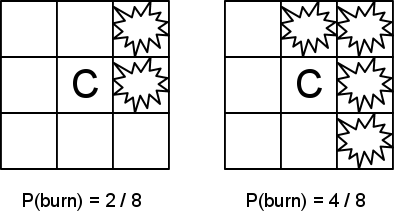
\includegraphics[width=0.5\textwidth]{solution/graphics/fire-probability.png}
\caption{Probability that fire will spread to a cell C on the grid without fire.}
\label{fig:fire-probability}
\end{figure}

The simple probability calculation was later extended to account for wind. Since wind can blow away smoke and heat, wind direction and magnitude directly affects how much impact each neighboring cell would have on C. To simulate this, each neighboring cell used a portion of the wind vector to produce a weight of impact. The sum of all these weights divided by a total weight became the new probability calculation in the fire spreading algorithm.

Humidity was implemented after wind. Humidity affects how fast fire spreads. It was implemented as a global value and had the same value for each cell. With this simplicity, we only had to either increase or decrease the total weight used in the probability calculation to adjust the rate of fire spread.

\subsection{Sensing Data}
After simulating data with wind and humidity, the next step was to use mobile phone sensors to read this data. Even if the current situation was known through the simulation at all times, we were only supposed to know the situation by the mobile phone sensor readings. To simulate sensing, two additional algorithms were used.

The first algorithm was a walking algorithm to simulate that people walk around with the mobile phone sensors. This algorithm assumed that sensors already had a position in order to do the following. For each time step, there was a fifty percent chance for each sensor to move. Because there were eight different directions to walk in a grid, the sensor picked a random direction. If the neighboring cell in the picked direction was on fire, the sensor had to pick another direction. In all, this algorithm only handled the location of the mobile phone sensors in the simulation. The next step after placing the sensors was to do readings.

The second algorithm was a sensing algorithm to provide known data used by the crisis mapping system. Because heat and smoke moves in the direction of the wind, the resulting sensor readings highly depended on wind and the location of the fire. Consider the example in figure \ref{fig:sense-concept}. Given the same wind vector W and two different neighbors at relative positions V1 and V2, each neighbor contributes differently to the sensor in C. In this particular case, the wind either blow heat and smoke away from C or into C depending on which neighbor it is.

\begin{figure}[here]
\centering
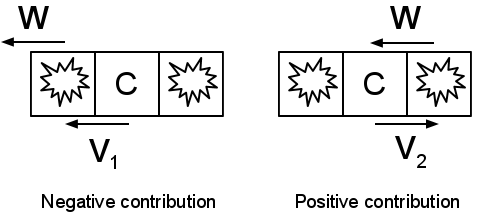
\includegraphics[width=0.65\textwidth]{solution/graphics/sense-concept.png}
\caption{Sensor readings are affected by wind and the positions of the neighboring emitting cells.}
\label{fig:sense-concept}
\end{figure}

The heat and smoke contribution to the sensor at C could be calculated as the sum of the cosine value of the angle between the wind vector W and the position vector for each neighbor. As shown in figure \ref{fig:sensor-contribution}, the cosine value could be divided into two ranges.

\begin{figure}[here]
\centering
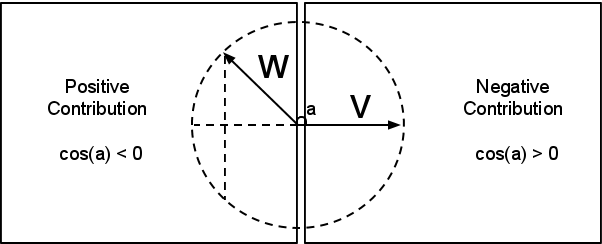
\includegraphics[width=0.65\textwidth]{solution/graphics/sensor-contribution.png}
\caption{Neighbor heat and smoke contribution is found by the cosine value between on wind W and neighbor position V relative to the sensor.}
\label{fig:sensor-contribution}
\end{figure}

The range [-1,0] was equal to positive contribution while the remaining [0,1] was equal to negative contribution. In case of a negative contribution, the contribution can simply be treated as 0 because heat and smoke would blow away from the sensor. To further simplify, by taking the absolute value of the positive contribution range [-1,0], the new range became [0,1] where 0 is the lowest and 1 is the highest contribution. This could be used as a coefficient to the heat and smoke emitted by this neighbor. Given that there are eight neighbors each indexed by i, the resulting mathematical formula used in the sensing algorithm is as follows:

\[
  c = \sum_{\substack i=1}^8\left\{
  \begin{array}{l l}
    |V_i \cdot W / \left(|V_i | \cdot |W| \right)| & \quad \text{if $V_i \cdot W < 0$}\\
   0 & \quad \text{if $V_i \cdot W >= 0$}\\
  \end{array} \right.
\]

\section{Fire Interpreter}
The fire interpreter's job is to receive input from the simulator and 
calculate values for the received cells. The calculated values are then posted to the visualizer. The advanced regression calculations are done by the library pyXGPR. This is a Gaussian Process Regression library implemented with Python. It produces a mean and a variance when used correctly. The first input parameter \textbf{X} is a list of points which tells where the training data is located. Another parameter \textbf{Y} contains the values to the training data. The last interpreter generated parameter \textbf{x star} contains the points where we want to find the mean and the variance. In addition to these parameters the library needs to be told what covariance functions pyXGPR should use to calculate the correlation between the cells in \textbf{X}, \textbf{Y} and \textbf{x star}. There is also added parameter values to these functions.
\\\\
The most basic use of pyXGPR is one dimensional (line regression) where \textbf{X} is the location and \textbf{Y} is the value. The fire interpreter uses regression in three dimensions where \textbf{x} and \textbf{y} are the map coordinates and an additional parameter \textbf{t} is for time. \textbf{t} is necessary to save earlier sensor data which later are utilized in predictions. It should also be mentioned that before this implementation, this was done by saving the best data. Best data is to be understood as the data which has the lowest variance. Data with lower variance would be applied to the saved map. This hack and the implementation of t is done because previous sensor data is important as long as they are weighted less than the newest sensor data. As time increases there will be sensor data covering a larger portion of the map, but the old sensor data will have less weight and thus giving new sensor data the opportunity to be taken into account. Figure \ref{fig:timeElapse} illustrates this.
\begin{figure}[here]
  \centering
      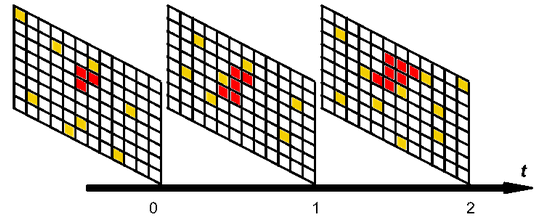
\includegraphics[width=0.5\textwidth]{solution/graphics/timeElapse.png}
  \caption{The fire interpreter saves the sensor data (yellow dots) and gives them a timestamp \textbf{t}. Earlier data is weighted less since the current \textbf{x star} and \textbf{X} has the same and last value for \textbf{t}. }
  \label{fig:timeElapse}
\end{figure}
\subsection{Performance}
The simulation map is 71 X 71 squares. GPR calculates the correlation between all points. This means pyXGPR creates huge matrices. As \textbf{t} increases the matrices grow larger and thus the execution time rises. The first version of the program used more than 6 minutes to run on a normal laptop. To better the performance it was found necessary to locate some squares which did not need to be calculated. Cells containing sensors was therefore removed from \textbf{x star} since the values were already there. With the introduction of \textbf{t}, the matrices became larger and execution time rose and once again it was necessary to find some steps to improve the performance. For a cell to be added to \textbf{x star} it had to be close to sensor which communicated fire. This was done by finding the euclidean distance between all cells which had no value and all sensors which communicated fire. This reduced the number of points in \textbf{x star} significantly. As time increases Another measure taken to reduce the execution time was to save cells which was calculated to be on fire. From these the euclidean distance to all points were calculated and if they were within a certain distance they would be added to \textbf{x star}.
\\\\
Before the interpreter posts the calculated data to the visualizer it converts the mean values to discrete values which is used in the visualizer to decide how intence the fire is burning. A threshold to determine if there should be fire is set, but can be difficult to determine as time progresses. The input values for sensors sensing fire is $0 $ to $10$, while sensors which are not sensing fire is converted from $ 0 $ to $ -1 $. The reason for the conversion is to get some more distance between fire and not fire. The fire threshold is set low to make sure all the realistic fire is covered.
\\\\
\subsection{Changes in pyXGPR kernel to support wind}
The simulation use wind as a crucial parameter to decide where the fire is spreading. Wind is therefore clever to use in the interpretation process. To make it a useful parameter the kernel in pyXGPR has been edited. The kernel contains all the different covariance functions and noise functions. The modification has been done in the function which measures the squared distance between two points. The squared distance is measured by creating two matrices for each dimension. In the fire interpreter these dimensions are \textbf{x}, \textbf{y} and \textbf{t}. One matrix containing all sensor data is deducted from a matrix containing all the uncalculated data. The dimensional result is multiplied with itself and added to a distance matrix. All dimensional results are added to the distance matrix. 
\\\\
\begin{eqnarray}
\theta = cos^{-1}\left(\dfrac{vector_{ij} \times windVector}{\|vector_{ij}\| \times \|windVector\| } \right) 
\label{eq:int-angle}
\end{eqnarray}
\begin{eqnarray}
weight = \dfrac{\theta}{\pi}
\label{eq:weight}
\end{eqnarray}
\begin{eqnarray}
\begin{bmatrix} distance_{11} & distance_{1j} \\ distance_{i1} & distance_{ij} \end{bmatrix} \times 
\begin{bmatrix} weight_{11} & weight_{1j} \\ weight_{i1} & weight_{ij} \end{bmatrix}
\label{eq:hadamard}
\end{eqnarray}
\\\\
Before these calculations the interpreter implementations in this function creates a weight matrix which has the same column and row values as the distance matrix. This weight is calculated with the forumula in \ref{eq:weight}. The Hadamard\cite{hadamard} product (see equation \ref{eq:hadamard}) of these two matrices is returned as the new distance matrix. 
\\\\
Where $ vector_{ij} $ is the vector from sensor position $i$ to uncalculated position $j$. The weight is further normalized to better fit the wind. If $ vector_{ij} $ is between $ 90^{\circ} $ and $ 180^{\circ} $ the weight will be normalized to larger than one and less than one if the angle is less than $ 45^{\circ} $. The values in the weight matrix is multiplied with the values in the distance matrix to create a hadamard\cite{hadamard} product. $ vector_{ij} $ in the weight matrix is multiplied with $ vector_{ij} $ in the distance matrix. This modifies the distance matrix where some values are reduced and some are increased, determined by their vector direction. The correlation of cells looks at the distance between them. Therefore decreased distance to a sensor sensing fire gives a cell a higher probability of being on fire. Sensors which does not detect fire will have a weight of one.
\subsection{Unexpected predictions with wind}
\label{wind-problem}
\begin{figure}[here]
  \centering
      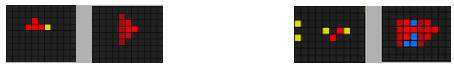
\includegraphics[width=1.0\textwidth]{solution/graphics/wind-problem.png}
  \caption{The left image illustrates when wind is used in predicting fire, while the right image illustrates the faults with a pure wind implementation. The blue dots are where the there should have been predicted fire.}
  \label{fig:wind-problem}
\end{figure}
The implementation of wind is working, but has some drawbacks. The first image in figure \ref{fig:wind-problem} illustrates how the fire is predicted when the wind is blowing from the east. The spread starts where the sensor is located and continuous in the shape of a triangle towards west. This looks good in the first image, but the second image illustrates the drawbacks. The wind is still blowing from the east and the two sensors detecting fire are on a horizontal line. The right tips of the predicted fire is where the sensors are located. The blue squares is used to highlight where there should have been predicted fire. This situation occurs because the blue squares are closest to the second sensor. The vector which goes from the second sensor to the any of blue square has an angle which is more than $ 45^{\circ} $ when compared to the wind vector which is $ \left[-1,0\right] $. Problems with predicting the middle part of the fire can occur when the the size of the predicted fire is becoming quite large. To solve both these problems there has been developed two solutions which have been tested with varying results. The first solution looks at the correlation between all sensors sensing fire while the second solution uses some techniques found in graphical programming. Another approach to these problems would be to use dynamic parameters. As the fire progressed the parameters would change in accordance to the size of the fire. But problems arises with such a solution as well. The edge of the fire would be more likely to be smudged out and it would in some cases predict fire in areas where there were no fire.
\subsubsection{Solution 1 to unexpected predictions with wind}
Burning sensor correlation was one approach to solve the problem when applying wind. It creates a list of all sensors which are sensing fire. Each element in the list has vectors to all other sensors communicating fire. In figure \ref{fig:burning-sensor-correlation} the green triangle is an uncalculated point while the numbered red circles are sensors sensing fire. There are vectors from sensor 1 to all other sensors sensing fire and a vector to the green triangle. This is an illustration of one of the entries in this list. The basis for this theory is that there is probably actual fire between the sensors. The blue vector compares direction with all the black vectors, see \ref{eq:int-angle}. It finds the black vector which has the most similar direction and check if it is within a certain threshold. If this comes out positive the distance for this point to sensor one will be multiplied with a number less than one, else it would be multiplied with one.
\begin{figure}[here]
  \centering
      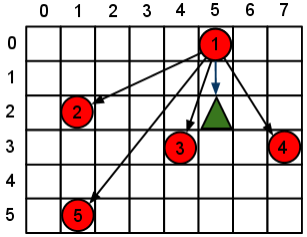
\includegraphics[width=0.4\textwidth]{solution/graphics/burning-sensor-correlation.png}
  \caption{All sensors (red) are sensing fire and sensor one has a vector to all other vectors sensing fire. The green triangle is an uncalculated point. Burning sensor correlation looks for the black vector which has the most similar angle to the closest blue vector.}
  \label{fig:burning-sensor-correlation}
\end{figure}
This approach has a fault. When a situation like \ref{fig:wind-problem} (second image) occurs it would predict fire against the wind. The burning sensor correlation would neutralize the added wind to such a degree that it was removed. The complexity with this solution is high and thus the execution time rises fast as \textbf{t} increases and the fire interpreter uses more data. As this solution was developed it would handle multiple fires badly.
\subsubsection{Solution 2 to unexpected predictions with wind}
In the second approach to solve the wind and filling issues, components from computer graphics were used. The outer boundary of the sensors sensing fire was chosen. The shape will be a convex polygon. Uncalculated cells within this polygon will have a higher probability of being on fire in the prediction. As in the burning sensor correlation implementation it is assumed its a higher probability of being fire between sensors sensing fire.
\begin{figure}[here]
  \centering
      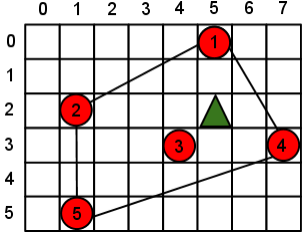
\includegraphics[width=0.4\textwidth]{solution/graphics/graphical-boundary.png}
  \caption{Locates all cells within the boundary.}
  \label{fig:graphical-boundary}
\end{figure}
To locate all the outer cells Graham's scan \cite{graham} was applied. When these points were found Bresenham's\cite{bresenham} line algorithm was used to find the in between cells. The result was all cells which the lines covered in figure \ref{fig:graphical-boundary} was retrieved. After this a scan line fill algorithm was used to find all the cells within the polygon. These steps resulted in a list of cell positions. This list was used when calculating the wind in accordance to wind direction. If the cell to be evaluated was inside this polygon the weight was multiplied with a number lower than one. This solution is also much faster than the first one. The Graham's scan and Bresenham's line algorithm was used as third party code, meaning we did not implement them. But the scan line algorithm was implemented in the kernel. Currently it does not handle multiple fires. If the two fires started at different \textbf{t} it could be possible to walk on predicted fire from one sensor to all the others.

\chapter{Discussion}
\section{Results}
The results are divided into two groups, simple simulation and advanced simulation. The results addressed in this section are reasonably representative for the average results.
\subsection{Results with simple simulation}
The simple simulation is characterized by sensors being spread relatively even throughout the map. The rule is that a sensor cannot touch another sensor. When using the simple simulator each sensor can only sense its closest neighbours. 
\\\\
Figure \ref{fig:simple-results1} illustrates the success of the fire interpreter. The light green color is where the actual fire is and where the interpreter predicted it to be. Therefore the color of success. The dark green color is area where the interpreter thought it would be fire, but was not. The red parts are the actual fire which the interpreter did not predict. 
\begin{figure}[here]
  \centering
      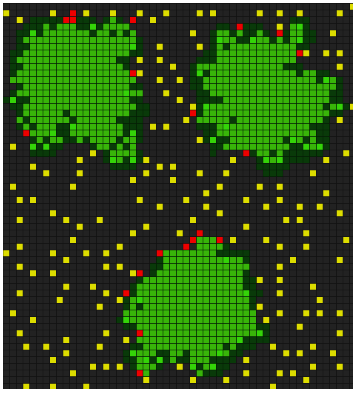
\includegraphics[width=0.7\textwidth]{discussion/graphics/results-simple-compare.png}
  \caption{The intense green is where the fire interpreter predicted correctly. The dark green is where the fire interpreter thought it was fire, but it was not. Red dots are where there actually was fire, but the predictor was unable to predict it.}
  \label{fig:simple-results1}
\end{figure}
\subsection{Results with advanced simulation}
The advanced simulation mimics the effect of humidity and wind has on a fire. The sensors are spread more randomly than in the simple simulation. They can also sense with a larger range. The default is two cells. The fire interpreter used the wind add-on in the kernel in the successful tests, while it was turned off in the tests which did not have too good results. There are a number of parameters which has been tweaked to get good results. These different parameters makes it more difficult to get an accurate prediction. Figure \ref{fig:wind-advanced-bresenham-large} illustrates the predicted fire on top of the actual fire when the wind is blowing from west.  
\begin{figure}[here]
  \centering
      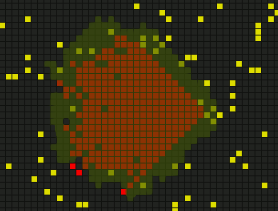
\includegraphics[width=0.5\textwidth]{discussion/graphics/wind-advanced-bresenham-large.png}
  \caption{The dark green overlay is where the fire interpreter predicted the fire to be. The red covered by the green overlay is where the fire interpreter predicted correctly and the red dots without any overlay is where there was fire, but did not predict.}
  \label{fig:wind-advanced-bresenham-large}
\end{figure}
The prediction is covering a larger area than the actual fire. This is because the sensors are sensing 2 cells away. In figure \ref{fig:wind-advanced-bresenham-large} this can be observed with the right most predicted fire. The two sensors which lays beneath the right most predicted area is sensing fire and therefore the prediction is set from this point. The first cells north and south of this area has also been calculated to be on fire. This is because of Bresenham’s line algorithm which interprets these two cells to be on the outer boundary of the sensors sensing fire. The algorithms from computer graphics is used to make sure there are no holes inside the predicted fire and to prevent wind problem (chapter \ref{wind-problem}).
\begin{figure}[here]
  \centering
      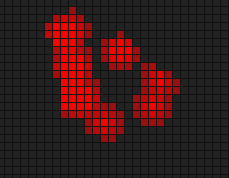
\includegraphics[width=0.5\textwidth]{discussion/graphics/advanced-without-wind-and-bresenham.png}
  \caption{Wind and graphical algorithms disabled in the advanced simulation creates holes and shows a lack wind direction.}
  \label{fig:advanced-without-wind-and-bresenham}
\end{figure}
\\\\
Figure \ref{fig:advanced-without-wind-and-bresenham} illustrates what is happening when wind and the graphical algorithms are disabled. Within the domain of the advanced simulation the results achieved with wind and the graphical algorithms. The prediction with this set up reproduces the shape of the actual fire with a satisfactory result. The area of the shape is larger than the actual fire. The philosophy was always to air on the side of safety. Meaning that the fire interpreter aimed to detect all fires and as such a few false positives were deemed to be acceptable.
\section {Practical Issues}
There are several practical issues that arises if this system should be put into motion. Collecting sensor data from a mobile phone and sending it to the crisis mapping system creates huge security and privacy issues. Personal data, like location and private conversations, may be useful in mapping a crisis, nevertheless the program should endeavour to protect the user and not disclose any information that is not relevant. In addition, the collected data should be transferred as fast as possible, over a secure connection, from the phone to the crisis mapping system to allow the program to react to new sensor readings as quickly as possible.

The system will always rely on sensors and people carrying a mobile phone capable of sensing. People will spectate on fires, but they will do it outside range of the heat and smoke. If it is blowing in one direction, the smoke and heat will drive people away from one side of the fire, meaning that there will not be sensor readings around the fire after they have moved away.

The mobile phone sensing scheme as with most other schemes, there are limitations to what is possible to achieve. Firstly, the crisis mapping system cannot account for human behavior. When a fire crisis occurs, people need to have a mobile phone with sensors available at that time, and people need to keep the mobile phone sensors close to the crisis situation. The further away the reading is made from the fire, the lower heat and smoke intensity would be read. Even if people would spectate the fire, they would do so away from harmful intensity. In all, this means that there is less good data to work with.
\chapter{Conclusion}

\clearpage
\addcontentsline{toc}{chapter}{Acknowledgments}
\chapter*{Acknowledgments}
\vspace{1.0in}
We would like to thank our supervisors Folke Haugland and Jaran Nilsen for their constructive feedback that has led to progress in times when the project was at a stand still. We would also like to thank Integrasco for letting us use their office to store the server and work in, and University of Agder for lending us the server.\\\\

02 june 2011\\
{University of Agder}\\
\newpage

\addcontentsline{toc}{chapter}{References}

\begin{thebibliography}{4}
\bibitem{graham} Alejo Hausner, CS Department, Princeton University
 \emph{http://www.cs.princeton.edu/courses/archive/spr10/cos226/demo/ah/GrahamScan.html (2011).} Prentice Hall
 
\bibitem{hadamard} Teknomo K. Hadamard Product. 2011. Available from \url{http://people.revoledu.com/kardi/tutorial/LinearAlgebra/HadamardProduct.html} 

\bibitem{bresenham} Flanagan C. The Bresenham Line-Drawing Algorithm. 2011. Available from \url{http://www.cs.helsinki.fi/group/goa/mallinnus/lines/bresenh.html} 

\bibitem{normal-dist} Inductiveload. Normal Distribution: curve. 2008. Available from \url{http://en.wikipedia.org/wiki/File:Normal_Distribution_PDF.svg} 
\bibitem{length-parameter} Wallach H. M. Introduction to Gaussian Process Regression: curve. 2005. Available from \url{http://www.cs.umass.edu/~wallach/talks/gp_intro.pdf} 

\bibitem{simple-covariance} Ebden M. Gaussian Processes for Regression: A Quick Introduction. aug 2008. Available from \url{http://www.robots.ox.ac.uk/~mebden/reports/GPtutorial.pdf} 


\bibitem{intro-to-gpr} Wallach H. M. Introduction to Gaussian Process Regression. jan 25, 2005. Available from \url{http://www.cs.umass.edu/~wallach/talks/gp_intro.pdf} 

\bibitem{fire-tirangleimage} Wikipedia,       \url{http://upload.wikimedia.org/wikipedia/commons/2/20/Fire_triangle.svg}, des 13, 2011

\bibitem{irevol} Patrick Meier, \underline{iRevolution} \url{http://irevolution.net/2011/01/20/what-is-crisis-mapping/} Posted on:jan 20, 2011, Visited on: des 14, 2011

\bibitem{mobsurv} Nicholas D. Lane, Emiliano Miluzzo, Hong Lu, Daniel Peebles, Tanzeem Choudhury,
and Andrew T. Campbell, Dartmouth College, \underline{IEEE Communications Magazine} \url{http://ieeexplore.ieee.org/stamp/stamp.jsp?tp=&arnumber=5560598 } Release: September 2010, Visited on: des 14, 2011

\bibitem{filmcrisis} Alison Stewart, "Need to Know", \underline{Crisis Mapping}, Premier date: may 13, 2011, \url{http://gis-techniques.blogspot.com/2011/05/new-way-of-mapping-crisis-mapping.html}

\bibitem{usha} "Ushahidi" \url{http://www.ushahidi.com/About-us} Visited on: des 14, 2011

\bibitem{springlink} Iizuka K ,Iizuka Y,Yoshida K, \emph{A Real-time Disaster Situation Mapping System for University Campuses}, \url{http://www.springerlink.com/content/0302-9743/?k=crisis+mapping} Publish date: 2011 Visited on: des 15, 2011

\bibitem{gitvers} "Version control glossary", \underline{What is version control} \url{What is version control} Visited on: des 14, 2011

\bibitem{gitis} "git the fast vesion control system", \underline{Git is...} \url{http://git-scm.com/}, Visited on: des 14, 2011

\bibitem{gausreg} Ebden M. \underline{Gaussian Processes for Regression: A Quick Introduction} Publish date: August 2008, \url{http://www.robots.ox.ac.uk/~mebden/reports/GPtutorial.pdf}, Visited on: des 15, 2011

\bibitem{intgausreg} Wallach H. M. \underline{Introduction to Gaussian Process Regression}
Publish date: January 25,2005
\url{http://www.cs.umass.edu/~wallach/talks/gp_intro.pdf}, Visited on: des 15, 2011

\bibitem{firebev} "Fire ecology and management", \underline{Fire Behaviour}, \url{http://learnline.cdu.edu.au/units/sbi263/fundamentals/behaviour.html}
Visited on: des 14, 2011, Last modified: aug 09, 2005

\bibitem{firebas} "Natural Resources Canada", \underline{Fire Basics}, \url{http://fire.cfs.nrcan.gc.ca/questions-fire-feu-eng.php} Visited on: des 14, 2011
Last modified: jun 30, 2011

\bibitem{rateofspread} "Knowledge and Application", \underline{Rate of Spread}, \url{http://www.forestencyclopedia.net/p/p478} Visited on: des 14, 2011, Last modified: nov 14, 2008

\bibitem{wildfire} Stephen J. Pyne, Patricia L. Andrews, Richard D. Laven, \emph{Introduction to Wildland fire. 2nd ed.}, John Wiley and Sons. Inc. 1996: p.37
\url{http://books.google.no/books?id=yT6bzpUyFIwC&pg=PA37&dq=Rothermel%E2%80%99s+equation+have+been+the+basis+for+most+of+the+fire+spread+prediction+models&hl=en&ei=j-foTsi9Esj34QSIof33CA&sa=X&oi=book_result&ct=result&redir_esc=y#v=onepage&q=Rothermel%E2%80%99s%20equation%20have%20been%20the%20basis%20for%20most%20of%20the%20fire%20spread%20prediction%20models&f=false}

\bibitem{firemov} "Fire ecology and management in northern Australia", \underline{Topography}, \url{http://learnline.cdu.edu.au/units/sbi263/fundamentals/topography.html}, 
Visited on: des 15, 2011

\bibitem{fireslope} "Unit2: Topographic Influences on Wildland Fire Behavioir" \url{http://deved.meted.ucar.edu/fire/s290/unit2/media/graphics/slopeandfirebehav.jpg} Visited on: des 15, 2011

\bibitem{firetypeimage} "Fire ecology and management in northern Australia", \underline{Fire regime}, \url{http://learnline.cdu.edu.au/units/sbi263/fundamentals/regime.html}, Visited on: des 15, 2011

\bibitem{firetypeimage} "Fire ecology and management in northern Australia", \underline{Climate, vegetation and fire}, \url{http://learnline.cdu.edu.au/units/sbi263/ecology/climate.html}, Visited on: des 15, 2011

\bibitem{fireweather} "Fire ecology and management in northern Australia", \underline{Fire weather}, \url{http://learnline.cdu.edu.au/units/sbi263/fundamentals/weather.html}, Visited on: des 15, 2011

\bibitem{relvhum} National Wildlife Coordinating Group, \emph{FIRE EFFECTS GUIDE
}, \url{http://www.nwcg.gov/pms/RxFire/FEG.pdf}, Last modified: jun 21, 2001, Visited on: des 15, 2011. 

\end{thebibliography}

%\appendix
%	%%
%% This is file `appendix.sty',
%% generated with the docstrip utility.
%%
%% The original source files were:
%%
%% appendix.dtx  (with options: `package')
%% =============================================
%% IMPORTANT NOTICE:
%% This is a generated file.
%% 
%% It is subject to the same copyright conditions (see below)
%% as in the original file: appendix.dtx.
%% It may not be distributed without appendix.dtx.
%% 
%% Full documentation can be obtained by LaTeXing that original file.
%% Only a few abbreviated comments remain here to describe the usage.
%% =============================================
%% Copyright 1993-2005 Patrick W Daly
%% Max-Planck-Institut f\"ur Aeronomie
%% Max-Planck-Str. 2
%% D-37191 Katlenburg-Lindau
%% Germany
%% E-mail: daly@linmpi.mpg.de
\NeedsTeXFormat{LaTeX2e}[1994/06/01]
\ProvidesPackage{appendix}
           [2005/10/30 2.2 (PWD)]
 % Adding this package redefines \appendix so that main counters for
 % figures, tables, equations are subnumbered under the appendix.
 % A \noappendix command is included so that things like bibliographies
 % may be called after the appendix with \section*. It resets the sectioning
 % commands. There should be no \section commands after this though.
 %
 % LaTeX2e options:
 %   mylang (default) -> keeps current \appendixname
 %   english, american  -> sets \appendixname to  `Appendix'
 %   german, austrian, french, esperanto -> translates \appendixname
 %   blank    -> suppresses the word `Appendix' with \appendix
 % Options processed in order given, default is mylang (no change)
 %-----------------------------------------------------------
\@ifundefined{iffigcaps}{}
  {\PackageWarningNoLine{appendix}
     {***********************************\MessageBreak
      This package read in after `figcaps'\MessageBreak
      There could be problems with sublabelled\MessageBreak
      figure and table numbers.\MessageBreak
      ***********************************}}
\DeclareOption{english}{\def\appendixname{Appendix}}
\DeclareOption{american}{\def\appendixname{Appendix}}
\DeclareOption{german}{\def\appendixname{Anhang}}
\DeclareOption{austrian}{\def\appendixname{Anhang}}
\DeclareOption{french}{\def\appendixname{Annexe}}
\DeclareOption{esperanto}{\def\appendixname{Apendico}}
\DeclareOption{blank}{\def\appendixname{}}
\DeclareOption{mylang}{\providecommand{\appendixname}{Appendix}}
\ExecuteOptions{mylang}
\ProcessOptions*
\let\orisection=\section
\let\theolds=\thesection
\let\theoldss=\thesubsection
\def\appendix{\par
  \if\@empty\appendixname \else  \section*{\appendixname} \fi
  \setcounter{section}{0}
  \setcounter{subsection}{0}
  \def\thesection{\Alph{section}}
  \def\thesubsection{\thesection\arabic{subsection}}
  \setcounter{secnumdepth}{4}
  \@addtoreset{equation}{section}
  \setcounter{equation}{0}
  \def\theequation{\thesection\arabic{equation}}
  \@addtoreset{figure}{section}
  \setcounter{figure}{0}
  \def\thefigure{\thesection\arabic{figure}}
  \@addtoreset{table}{section}
  \def\thetable{\thesection\arabic{table}}
  \setcounter{table}{0}
\def\@Alph##1{%
  \ifcase##1A\or A\or B\or C\or D\or E\or F\or G\or H\or I\or J\or
   K\or L\or M\or N\or O\or P\or Q\or R\or S\or T\or U\or V\or W\or X\or
    Y\or Z\else\@ctrerr\fi}
}
\def\noappendix{\setcounter{secnumdepth}{0}
  \global\let\section=\orisection
  \global\let\thesection=\theolds
  \global\let\thesubsection=\theoldss
}
%% 
%% <<<<< End of generated file <<<<<<
%%
%% End of file `appendix.sty'.

%	\include{acro}




%\bibliographystyle{IEEEtranS}
%\bibliography{bibliography}

\end{document}
